\noindent\begin{minipage}{7cm}
\begin{description}
\item[Objectif :] savoir spécifier une fonction.
\item[Syntaxe \python :] \mbox{}
\begin{Verbatim}
def nom(entrées) :
    """ 
    description
    jeux de tests
    """
    assert préconditions
    ...
    return sorties
\end{Verbatim}
\end{description}
\end{minipage}
\mbox{}\hfill
\begin{minipage}{8cm}
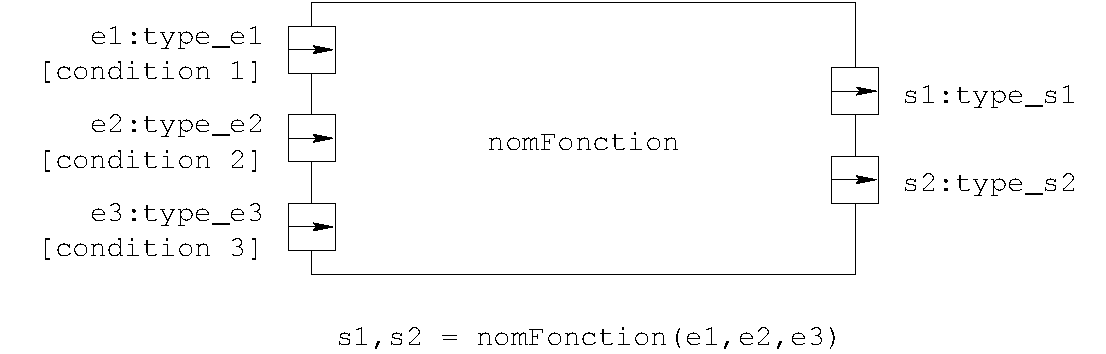
\includegraphics[width=8cm]{fonction-uml.pdf}
\end{minipage}
%\begin{tabular}{c}
%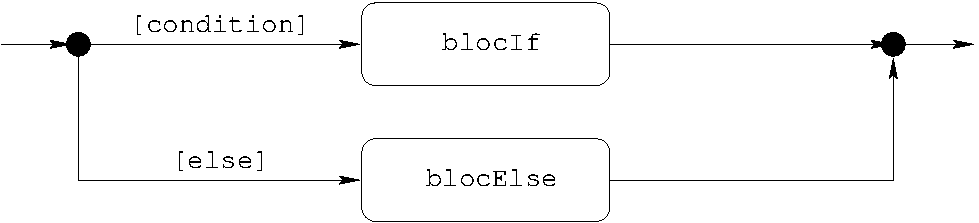
\includegraphics[width=6.5cm]{uml1.pdf}\\[3mm]
%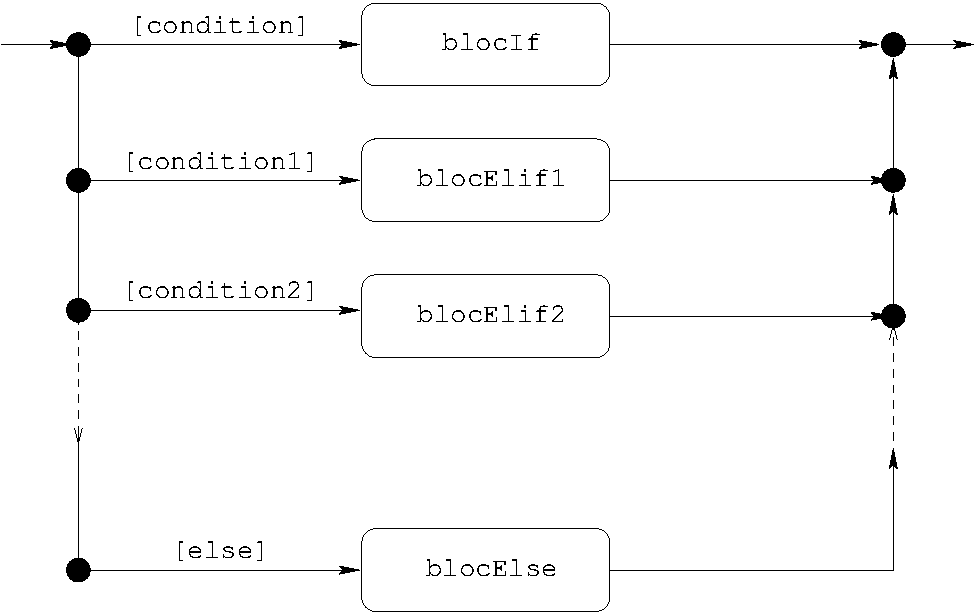
\includegraphics[width=6.5cm]{uml3.pdf}
%\end{tabular}

%-------------------------------------------------------------------------
\subsection{Exemple}
%-------------------------------------------------------------------------

\paragraph{Enoncé :} On dispose d'une recette de quatre-quarts aux pépites de chocolat
pour laquelle on veut séparer le « quoi » faire du « comment » faire.
\vspace*{2mm}

\noindent\begin{minipage}{9cm}
Ingrédients (pour 8 personnes) :
\begin{itemize}
\item 100 g de pépites de chocolat,
\item 200 g de beurre ramolli,
\item 200 g de sucre en poudre,
\item 3 \oe ufs,
\item 200 g de farine,
\item 1 pincée de sel.
\end{itemize}
\end{minipage}
\hfill
\begin{minipage}{6cm}
\centerline{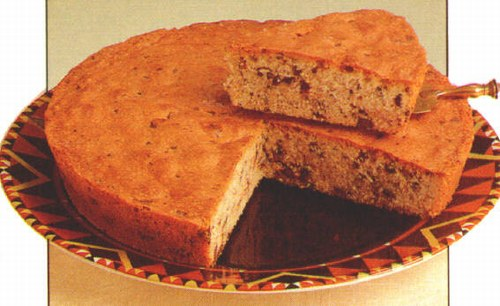
\includegraphics[width=6cm]{quatre-quarts-chocolat.jpg}}
\end{minipage}
\vspace*{2mm}

\noindent
Préparation ($\approx$ 30' + 45' de cuisson) :
\begin{itemize}
\item Préchauffer le four à 160°C (thermostat 5-6).
\item Travailler le beurre ramolli, mais non fondu, avec une spatule pour le rendre crémeux.
\item Ajouter progressivement le sucre et battre vigoureusement, le mélange doit être onctueux.
\item Casser les \oe ufs en séparant les jaunes des blancs. 
	Ajouter les jaunes à la préparation et mélanger.
\item Incorporer progressivement la farine tamisée puis les blancs battus en neige 
	avec une pincée de sel, en soulevant la pâte de bas en haut.
\item Ajouter les pépites de chocolat en mélangeant délicatement. 
\item Verser la préparation dans un moule à quatre-quarts beurré et fariné et 
	faire cuire 45 minutes à four chaud.
\end{itemize}

\paragraph{Méthode :} Distinguer la spécification de l'implémentation :
\begin{itemize}
\item la spécification d'un algorithme décrit ce que fait l'algorithme 
et dans quelles conditions il le fait;
\item l'implémentation d'un algorithme décrit comment fait l'algorithme 
pour satisfaire sa spécification.
\end{itemize}

\paragraph{Questions :} \mbox{}

\begin{question}[« quatre-quarts » : situations initiale et finale]\mbox{}
\begin{enumerate}
\item De quoi dispose-t-on avant de réaliser la quatre-quarts (situation initiale) ?
\item De quoi dispose-t-on après avoir réalisé le quatre-quarts (situation finale) ?
\end{enumerate}

\end{question}

Un algorithme est un mécanisme qui fait passer un « système » d'une « situation »
dite initiale à une « situation » finale. 
Le couple (situation initiale, situation finale) constitue une spécification de 
l'algorithme. 

\begin{question}[« quatre-quarts » : réalisation] 
Quelles actions doit-on effectuer pour réaliser le qua\-tre-quarts ?
\end{question}

La suite d'instructions qui permet de passer de la situation initiale à 
la situation finale constitue une implémentation de l'algorithme. 
Il peut exister plusieurs implémentations pour une même spécification.

%-------------------------------------------------------------------------
\subsection{Généralisation}
%-------------------------------------------------------------------------
Une fonction est un bloc d'instructions nommé et paramétré,
réalisant une certaine tâche. Elle admet zéro, un ou plusieurs 
paramètres et renvoie toujours un résultat.

Une fonction en informatique se distingue principalement de la 
fonction mathématique par le fait qu'en plus de calculer un résultat 
à partir de paramètres, la fonction informatique peut avoir des « effets de bord »: 
par exemple afficher un message à l'écran, jouer un son, 
ou bien piloter une imprimante.
Une fonction qui n'a pas d'effet de bord joue le rôle d'une expression
évaluable. Une fonction qui n'a que des effets de bord est appelée une procédure
et joue le rôle d'une instruction.

Une procédure est un bloc d'instructions nommé et paramétré,
réalisant une certaine tâche. Elle admet zéro, un ou plusieurs 
paramètres et ne renvoie pas de résultat.

\begin{question}[spécification d'une fonction : nommer]
Proposer un nom pour la procédure qui réalise un quatre-quarts aux pépites.
\end{question}

Les paramètres d'entrée d'une fonction sont les arguments de la fonction
qui sont nécessaires pour effectuer le traitement associé à la fonction.

Les paramètres de sortie d'une fonction sont les résultats retournés 
par la fonction après avoir effectué le traitement associé à la fonction.

\begin{question}[spécification d'une fonction : paramétrer]
Préciser les paramètres d'entrée et de sortie
de la procédure qui réalise un quatre-quarts aux pépites.
\end{question}

Les préconditions d'une fonction sont les conditions que doivent 
impérativement vérifier les paramètres d'entrée de la fonction
juste avant son exécution.

\begin{question}[spécification d'une fonction : protéger]
Quelles sont les conditions que doivent vérifier les paramètres d'entrée
de la procédure de réalisation du quatre-quarts ?
\end{question}

Un jeu de tests d'une fonction est un ensemble d'entrées-sorties associées
que devra vérifier la fonction une fois implémentée.

\begin{question}[spécification d'une fonction : tester]
Proposer un jeu de tests pour la procédure de réalisation du quatre-quarts.
\end{question}


L'algorithmique s'intéresse à l'art de construire 
des algorithmes ainsi qu'à caractériser leur validité, leur robustesse
leur réutilisabilité, leur complexité ou encore leur efficacité. Certaines 
de ces caractéristiques générales, en particulier la validité, la robustesse
et la réutilisabilité 
se concrétisent à la lumière des préconisations précédentes concernant 
la spécification d'une fonction.

\begin{enumerate}
\item La validité d'un algorithme est son aptitude à réaliser 
	exactement la tâche pour laquelle il a été conçu.

	{\em ie}: L'implémentation de la fonction doit être conforme aux jeux de tests.
\item La robustesse d'un algorithme est son aptitude à se 
	protéger de conditions anormales d'utilisation.

	{\em ie}: La fonction doit vérifier impérativement ses préconditions.
\item La réutilisabilité d'un algorithme est son aptitude 
	à être réutilisé pour résoudre des tâches équivalentes à celle pour 
	laquelle il a été conçu.

	{\em ie}: La fonction doit être correctement paramétrée.
\end{enumerate}


%-------------------------------------------------------------------------
\subsection{Applications}
%-------------------------------------------------------------------------
\begin{question}[prix d'une photocopie]\mbox{}
Spécifier la fonction qui calcule le prix $p$ de $n$ photocopies sachant que le reprographe
facture 0.10 \euro{} les 10 premières photocopies, 0.09 \euro{} les vingt suivantes et 0.08 \euro{} au-delà.
\end{question}

\begin{question}[somme arithmétique]\mbox{}
\begin{enumerate}
\item Spécifier la fonction qui calcule la somme $s = \sum_0^n u_k$ des $n$ premiers termes d'une suite arithmétique $u_k = a + kb$.
\item Proposer au moins deux implémentations différentes pour la spécification proposée.
	Classer ces implémentations par ordre de complexité croissante.
\end{enumerate}
\end{question}

%-------------------------------------------------------------------------
%\newpage
\subsection{Entraînement}
%-------------------------------------------------------------------------

%-------------------------------------------------------------------------
\subsubsection{Enoncé}
%-------------------------------------------------------------------------

\paragraph{Objectif :} spécifier une fonction connue (un « grand classique »).

\paragraph{Méthode :} procéder en 4 étapes : nommer, paramétrer, protéger, 
proposer un jeu de tests, en faisant évoluer à chaque étape la description 
de la fonction.

\paragraph{Vérification :} vérifier le jeu de tests gr\^ace à une implémentation connue.

%-------------------------------------------------------------------------
\subsubsection{Exemple}
%-------------------------------------------------------------------------
Soit à spécifier la fonction qui détermine les racines réelles d'un trinôme du 
second degré à coefficients réels ($ax^2 + bx + c$).

\paragraph{Méthode :} on avancera pas à pas en passant par les 4 étapes conseillées :
nommer, paramétrer, protéger, proposer un jeu de tests,
en faisant évoluer la description de la fonction en conséquence.

\begin{enumerate}
\item 
\begin{minipage}[t]{6cm}
\textbf{Nommer} la fonction à l'aide d'un identificateur suffisamment explicite.
Dans cet exemple, nous choisirons : \texttt{racinesTrinome}, avec pour description
«~détermination des racines d'un trinôme du second degré~».
\end{minipage}
\hfill
\begin{minipage}[t]{9cm}\footnotesize
\begin{lstlisting}
def racinesTrinome() :
    """
    determination des racines d'un 
    trinome du second degre
    """
    return
\end{lstlisting}
\end{minipage}
\vspace*{1mm}

\item 
\begin{minipage}[t]{6cm}
\textbf{Paramétrer} la fonction en entrée comme en sortie.
Ici, la fonction prendra trois arguments en entrée : les coefficients $a$, $b$ et $c$
du trinôme $ax^2 + bx + c$. En sortie, nous attendons une liste des racines obtenues : 
« racines : liste des racines du trinôme \texttt{a*x**2 + b*x + c}~».
La longueur de la liste retournée (\texttt{len(racines)}) indiquera le nombre de
racines obtenues (0, 1 ou 2).
\end{minipage}
\hfill
\begin{minipage}[t]{9cm}\footnotesize
\begin{lstlisting}
def racinesTrinome(a,b,c) :
    """
    racines = racinesTrinome(a,b,c)
    racines : liste des racines du 
              trinome a*x**2 + b*x + c
    """
    racines = []
    return racines
\end{lstlisting}
\end{minipage}
\vspace*{2mm}

\item 
\begin{minipage}[t]{6cm}
\textbf{Protéger} la fonction à l'aide de préconditions sur les paramètres d'entrée.
Ici, \texttt{a} doit être un réel (\texttt{type(a) is float}) non nul (\texttt{a != 0}), \texttt{b} et \texttt{c} des réels (\texttt{type(b) is float}, \texttt{type(c) is float}).
En \python, ces conditions seront testées à l'aide de l'instruction \texttt{assert}.
La description s'enrichit alors de ces conditions sur les paramètres d'entrée.
\end{minipage}
\hfill
\begin{minipage}[t]{9cm}\footnotesize
\begin{lstlisting}
def racinesTrinome(a,b,c) :
    """
    racines = racinesTrinome(a,b,c)
    racines : liste des racines du 
    trinome a*x**2 + b*x + c
    (a: float != 0, b: float, c: float)
    """
    assert type(a) is float and a != 0.0
    assert type(b) is float
    assert type(c) is float
    
    racines = []
    return racines
\end{lstlisting}
\end{minipage}
\vspace*{1mm}

\item 
\begin{minipage}[t]{6cm}
\textbf{Proposer un jeu de tests}
le plus caractéristique possible.
On testera notamment quelques identités remarquables :\\
$(x-d)^2 = 0 \Rightarrow x = d$, \\
$(x+d)^2 = 0 \Rightarrow x = -d$, \\
$(x^2 - d^2) = 0 \Rightarrow x = d$ ou $x = -d$. 
On testera également un cas où il n'y a pas de racines :\\
$(x^2 + d^2)$.

Ces couples d'entrées-sorties cohérentes seront testés en \python{}
à l'aide du module \texttt{doctest}.
\end{minipage}
\hfill
\begin{minipage}[t]{9cm}\footnotesize
\begin{lstlisting}
def racinesTrinome(a,b,c) :
    """
    racines = racinesTrinome(a,b,c)
    racines : liste des racines du 
    trinome a*x**2 + b*x + c
    (a: float != 0, b: float, c: float)
    
    >>> racinesTrinome(1.0,0.0,1.0)
    []
    >>> racinesTrinome(1.0,-2.0,1.0)
    [1.0]
    >>> racinesTrinome(1.0,2.0,1.0)
    [-1.0]
    >>> racinesTrinome(1.0,0.0,-4.0)
    [2.0, -2.0]
    """
    assert type(a) is float and a != 0.0
    assert type(b) is float
    assert type(c) is float
    
    racines = []
    return racines
\end{lstlisting}
\end{minipage}

\end{enumerate}

\vspace*{2mm}

\paragraph{Résultat :} la spécification \python{} du calcul des racines
du trinôme correspond à la version obtenue à la dernière étape de la 
méthode précédente
(étape 4 : « proposer un jeu de tests »).

\noindent\begin{minipage}{5cm}
Le diagramme \uml{} associé est donné ci-contre :
\end{minipage}
\hfill
\begin{minipage}{10cm}
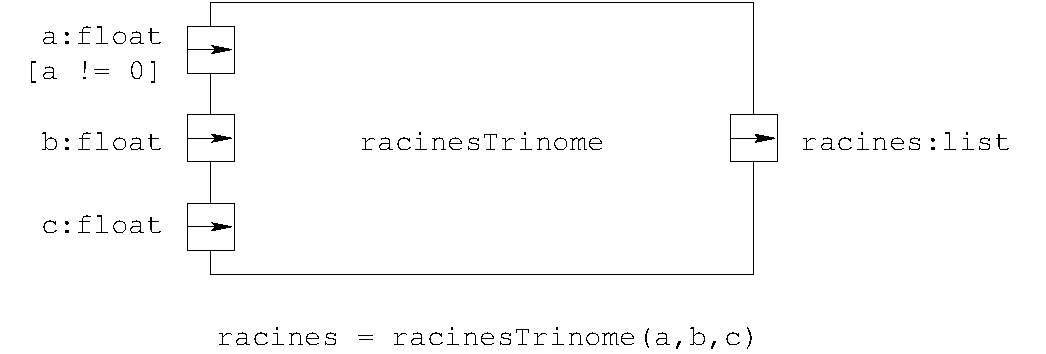
\includegraphics[width=9cm]{racines.pdf}
\end{minipage}

\paragraph{Vérifications :} la fonction sera testée une fois son implémentation
définie (voir par exemple le TD 2.31 page 70 du cours \cite{cours}) grâce aux 
lignes suivantes dans le fichier source :
\vspace*{3mm}

\noindent\begin{minipage}{4cm}
\begin{Verbatim}
if __name__ == "__main__":
    import doctest
    doctest.testmod()
\end{Verbatim}
\end{minipage}
\hfill
\begin{minipage}{9cm}
Lors de la compilation du fichier, l'interpréteur signalera toutes
différences observées entre le jeu de tests spécifié et les résultats 
effectifs obtenus en testant lui-même les instructions du jeu de tests.
\end{minipage}

%-------------------------------------------------------------------------
\subsubsection{Questions}
%-------------------------------------------------------------------------
Proposer une spécification\footnote{Les implémentations de 
ces fonctions ne sont pas demandées; on les trouvera 
dans le cours «~{Initiation à l'algorithmique}~» \cite{cours}.}
 pour les fonctions suivantes :

\noindent\begin{minipage}[t]{7cm}
\begin{enumerate}\setcounter{enumi}{0}
\item algorithme d'Euclide
\item coefficients du binôme
\item conversion en base $b$
\item courbe fractale de Koch
\item crible d'Eratosthène
\item développement limité de $sin(x)$
\item fonction factorielle
\item fonction puissance
\item intégration numérique
\item nombres de Fibonacci
\item palindrome
\item produit de matrices
\end{enumerate}
\end{minipage}
\hfill
\begin{minipage}[t]{7cm}
\begin{enumerate}\setcounter{enumi}{12}
\item produit mixte de vecteurs
\item racines du trinôme
\item recherche dichotomique
\item recherche séquentielle
\item tours de Hanoï
\item tracé d'un polygone régulier
\item tri bulles
\item tri fusion
\item tri par insertion
\item tri par sélection
\item tri rapide
\item zéro d'une fonction
\end{enumerate}
\end{minipage}

%-------------------------------------------------------------------------
\subsection{Révisions}
%-------------------------------------------------------------------------

$$\begin{tabular}{|ll@{ : }l|}
\hline
\textbf{Cours} & \cite{cours} & chapitre 3, sections 3.1 et 3.2 \\
\textbf{TD}    & \cite{td}    & exercices 3.3 à 3.5,  \\
\hline
\end{tabular}$$
